\documentclass{article}
\usepackage{graphicx}
\usepackage{caption}
\usepackage{subcaption}

\title{Report 5 - Gaussian Blur from CUDA}
\author{Le Nhu Chu Hiep}

\begin{document}
\maketitle

\section{Implementation}

\begin{itemize}
    \item Build new kernel function to perform convolution with blur kernel
    \item Reuse host logic of labwork 4 to run new kernel
\end{itemize}

\section{Result}

\subsection{Text Result}
\begin{verbatim}
USTH ICT Master 2018, Advanced Programming for HPC.
Warming up...
Starting labwork 5
labwork 5 CPU ellapsed 71.9ms
Block Size: 1024, Grid Size: 1900
labwork 5 GPU no shared mem ellapsed 16.2ms
Block Size: 1024, Grid Size: 1900
labwork 5 GPU shared mem ellapsed 17.0ms
labwork 5 ellapsed 17.0ms
\end{verbatim}

\subsection{Image Result}
\begin{figure}
        \begin{subfigure}{\textwidth}
            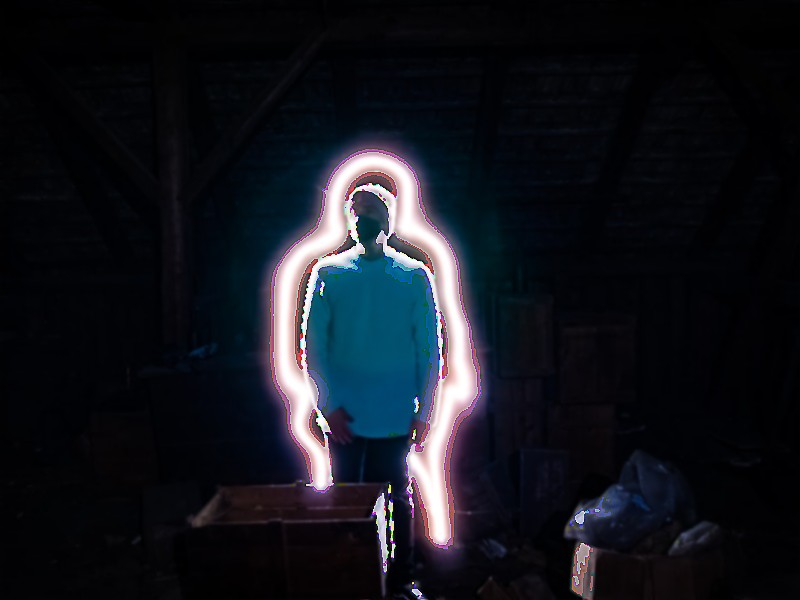
\includegraphics[width=\textwidth]{./labwork5-cpu-out.jpg}
            \caption{CPU Version}
        \end{subfigure}
        \begin{subfigure}[b]{0.5\textwidth}
            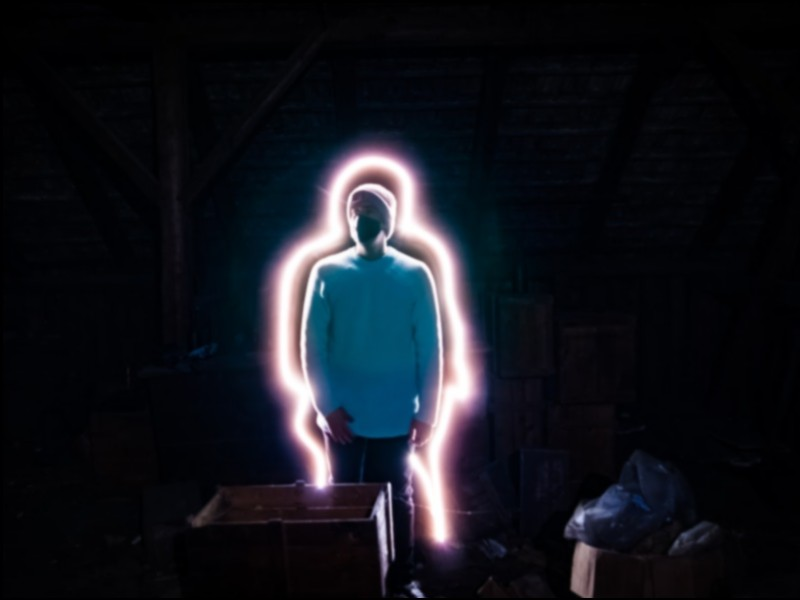
\includegraphics[width=\textwidth]{./labwork5-gpu-out-no-shared.jpg}
            \caption{GPU Without Share Mem Version}
        \end{subfigure}
        \begin{subfigure}[b]{0.5\textwidth}
            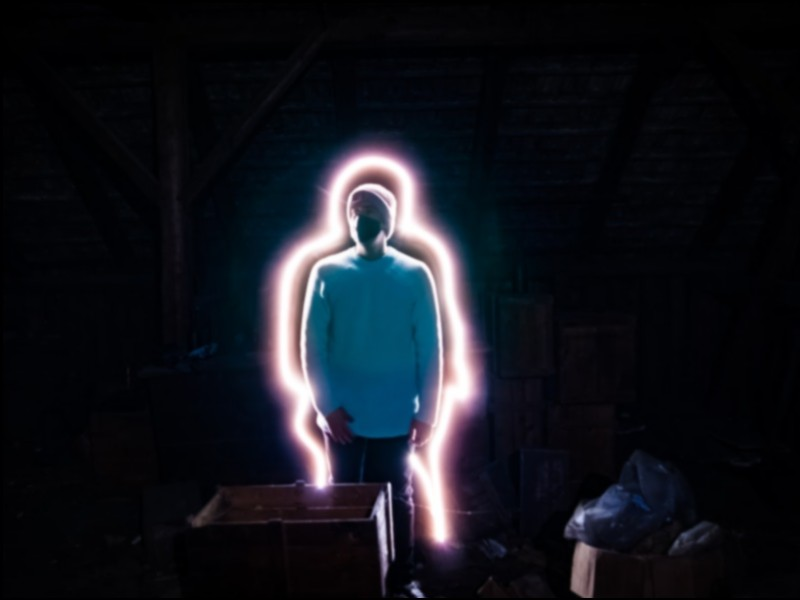
\includegraphics[width=\textwidth]{./labwork5-gpu-out-shared.jpg}
            \caption{GPU With Share Mem Version}
        \end{subfigure}
        \caption{Result Images}
\end{figure}

\end{document}
